%!TEX root = ../../../main.tex
%%---------------------------------------------------------------------------
\section{Hardware}
\label{sec:rc_hardware}
%%---------------------------------------------------------------------------
The following hardware elements was provided in each robot cell:

\begin{itemize}
	\item Kuka KR6 Robot
	\item PG70 Gripper
	\item Conveyor Belt with 3 phase 240V Motor
	\item ABB (ACS150-01E) Frequency Converter
	\item ABB (PM554) Programmable Logic Controller(PLC) for conveyor control
	\item SICK (M4000) Laser safety fence
	\item HD Webcam for Lego brick detection in 2D
	\item Kuka touch screen for HMI
\end{itemize}

The set-up for involved components will be discussed in details where appropriate. 

\subsection{Modifications}
The conveyor belt required some changes to be able to handle and control the flow of Lego bricks. First a funnel, see figure \ref{fig:funnel}, was added as a tip-off location for the mobile robot.

  	\begin{figure}[H]
        \centering
        \begin{subfigure}{0.48\textwidth}
			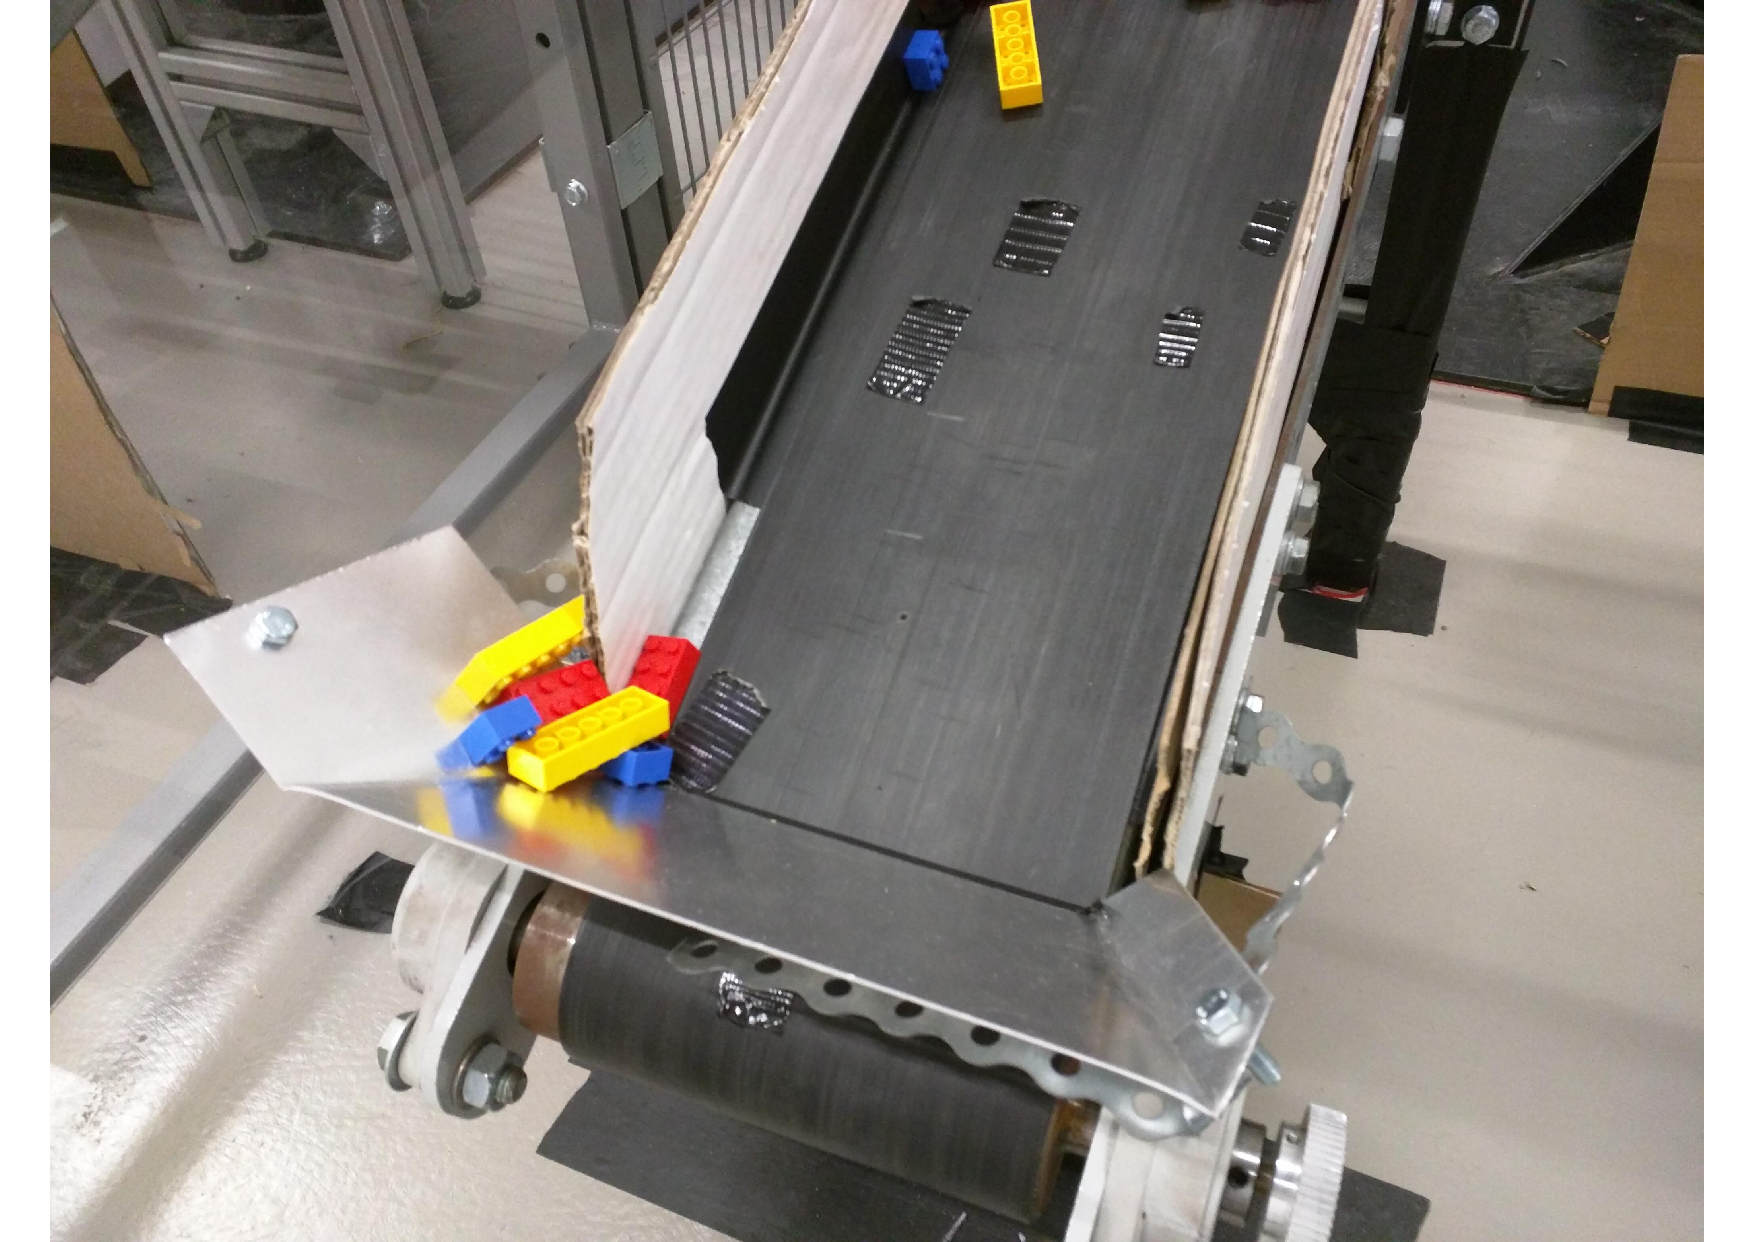
\includegraphics[width=1\textwidth]{funnel_rc}
			\caption{Funnel at delivery point for the mobile robot}
			\label{fig:funnel}
        \end{subfigure}
        \hspace{10pt}
        \begin{subfigure}{0.48\textwidth}
			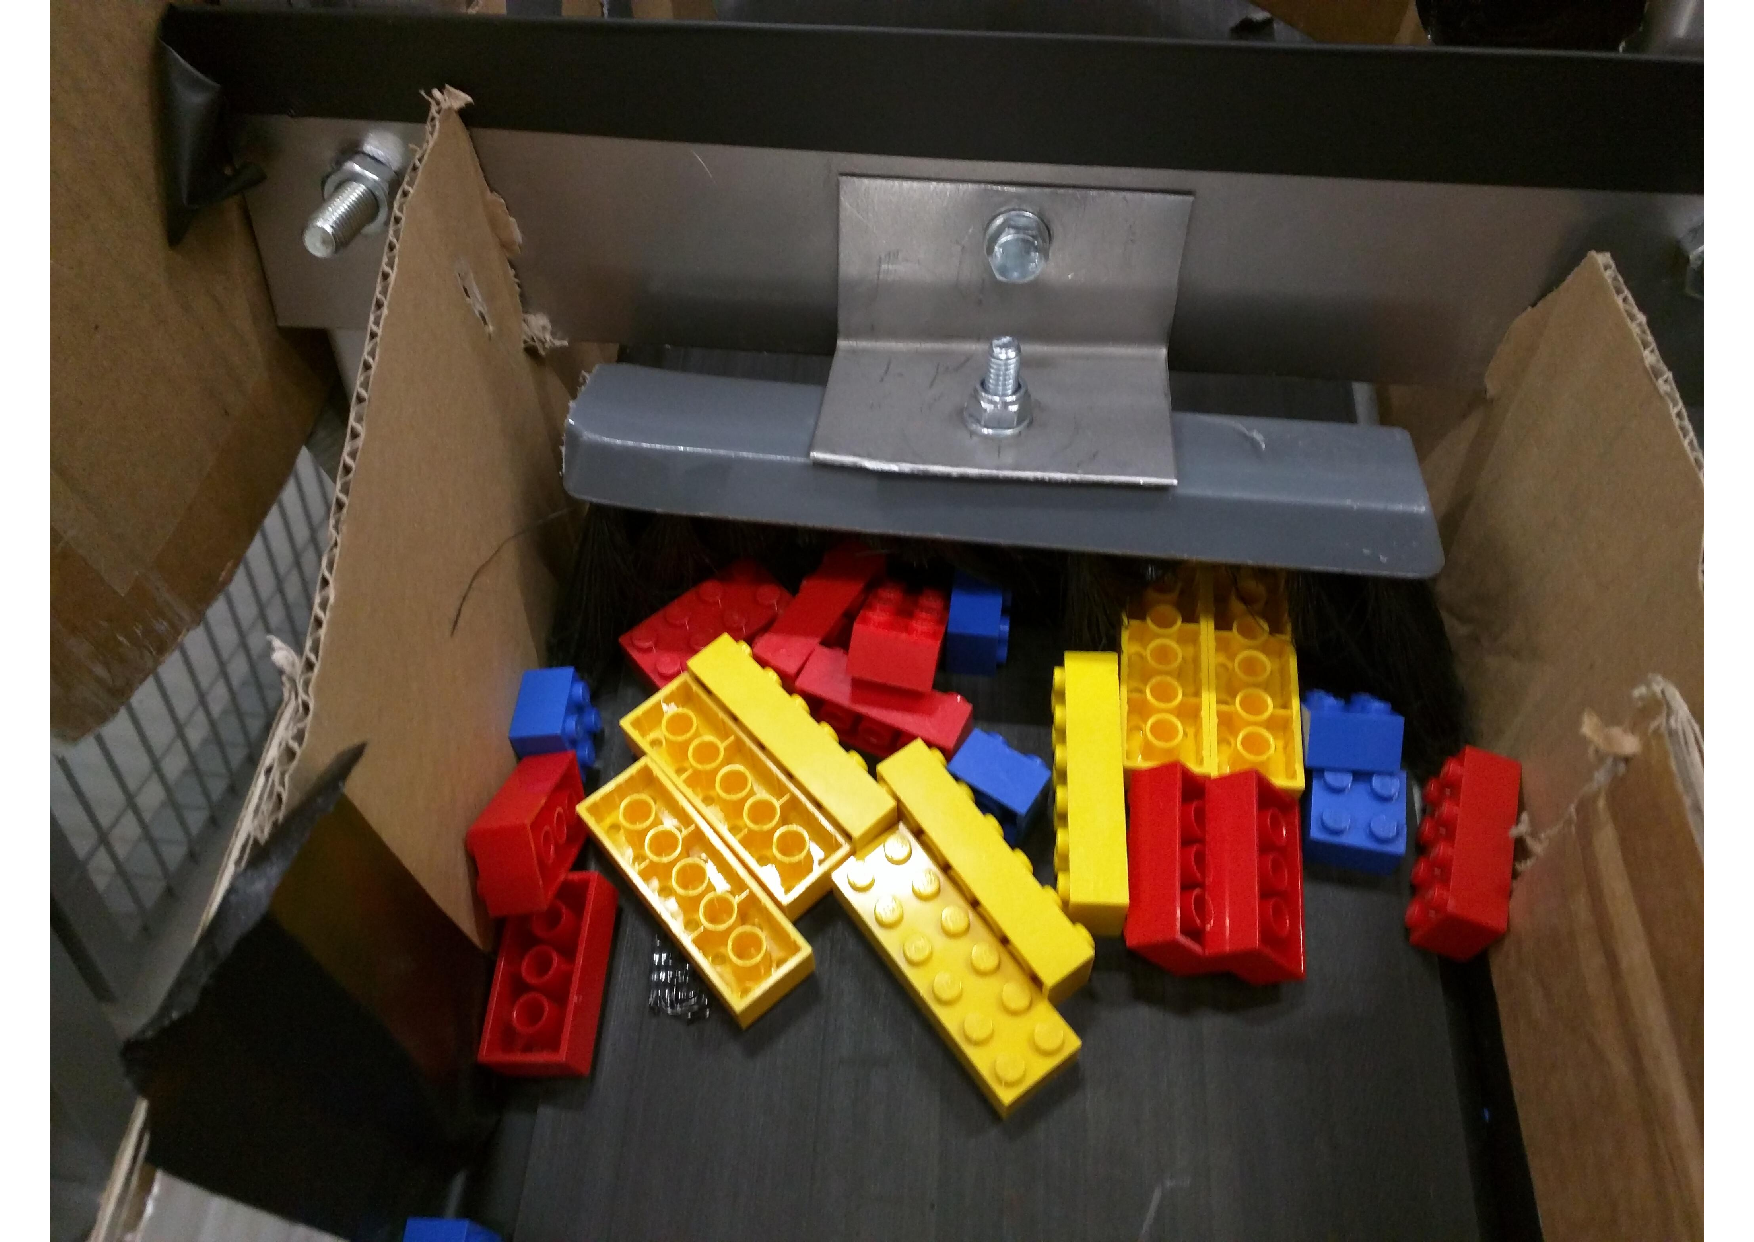
\includegraphics[width=1\textwidth]{brush_rc}
			\caption{Brush system to de-cluster the bricks}
			\label{fig:brush}
    \end{subfigure}
    \caption{Example of conveyor modifications}
    \end{figure}

Secondly, to avoid clustering and multiple layers of bricks a passive system consisting of a brush and cardboard was invented as shown in figure \ref{fig:brush}.

To provide the necessary friction to go through the system, duct tape was added at random places to the conveyor belt. See figure \ref{fig:duct_tape}.

  	\begin{figure}[H]
        \centering
        \begin{subfigure}{0.48\textwidth}
			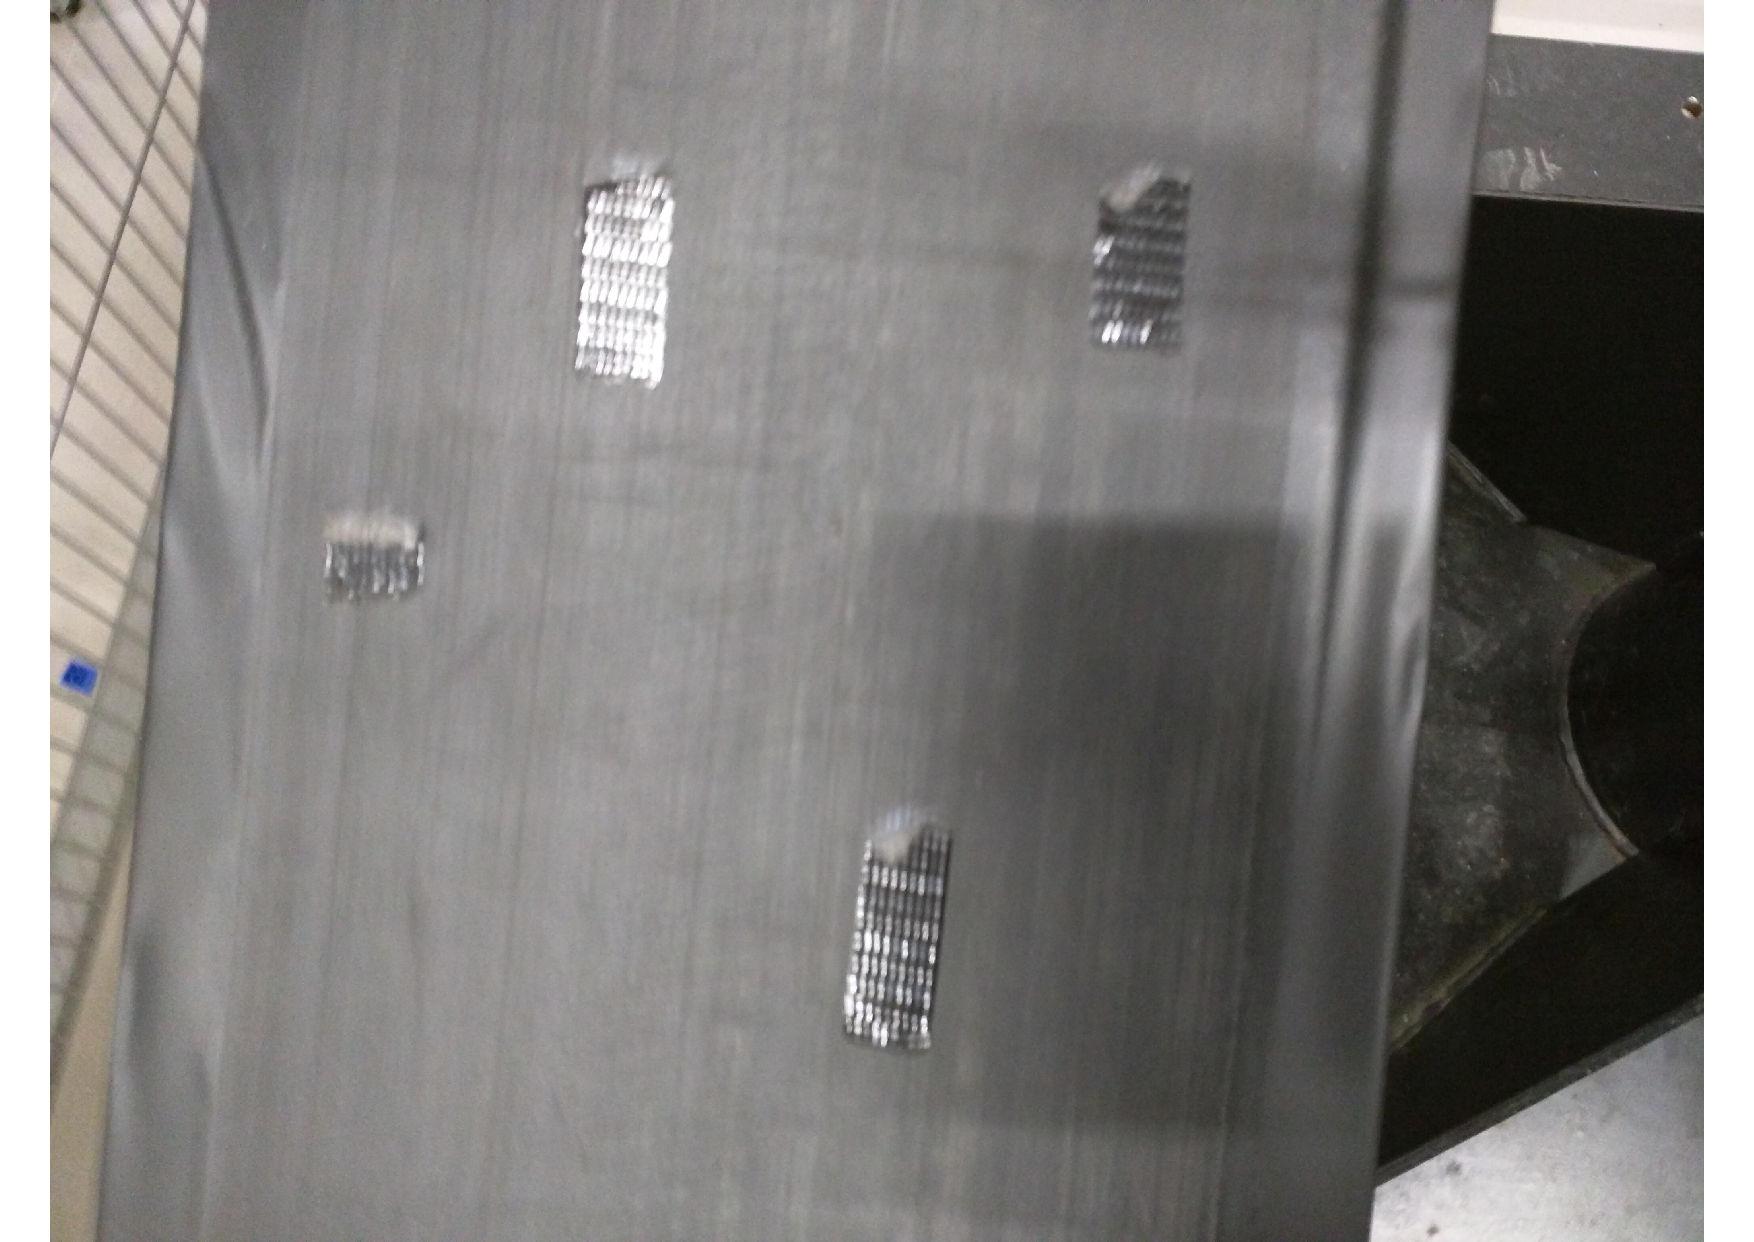
\includegraphics[width=1\textwidth]{duct_tape_rc}
			\caption{Duct tape mounted to conveyor belt}
			\label{fig:duct_tape}
        \end{subfigure}
        \hspace{10pt}
        \begin{subfigure}{0.48\textwidth}
			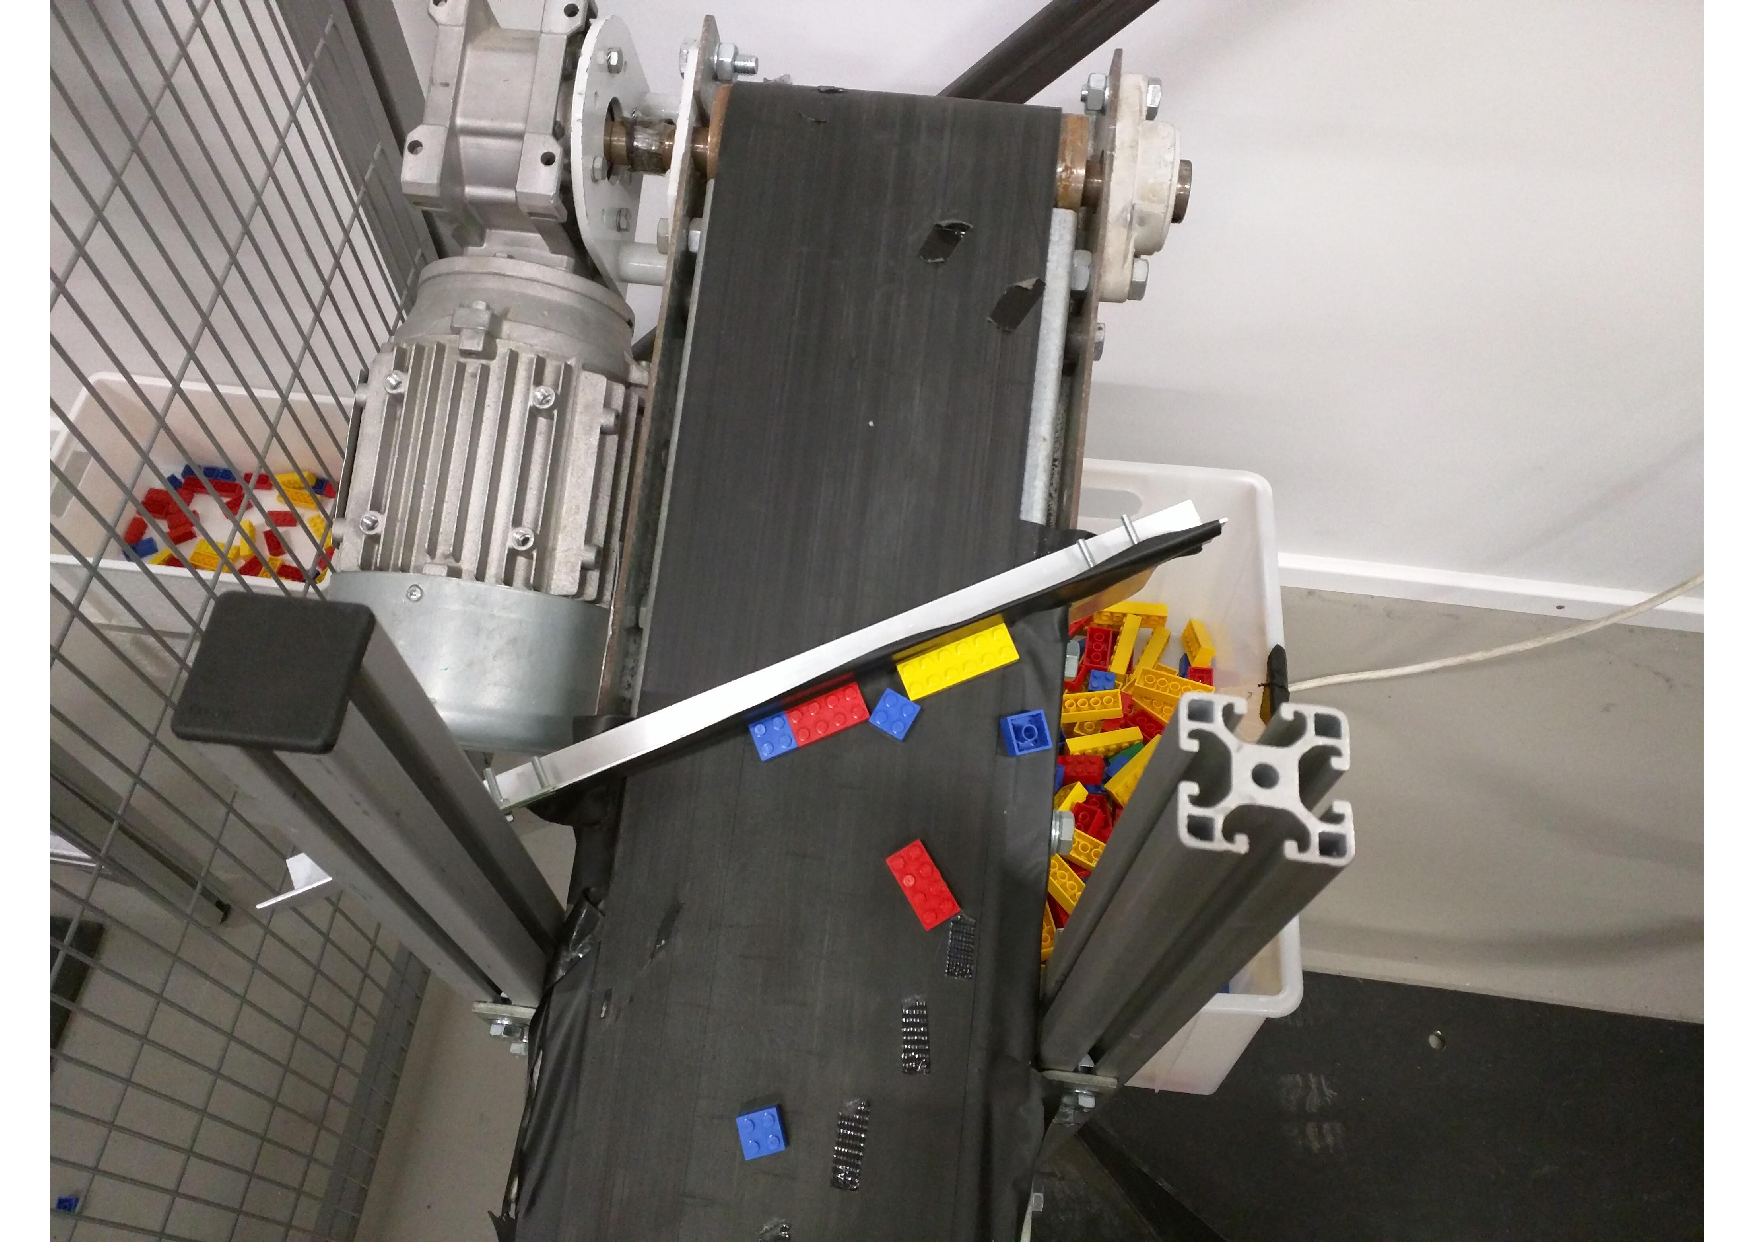
\includegraphics[width=1\textwidth]{slider_to_box}
			\caption{Slider to ensure spare bricks to fall into the box}
			\label{fig:slider}
    \end{subfigure}
    \caption{Example of conveyor modifications}
    \end{figure}

Finally, to avoid unwanted bricks on the floor, a passive slider was mounted near end of the conveyor belt. This allows the bricks to fall into a well placed box and collected at a later time. See figure \ref{fig:slider} 
